\documentclass[conference,12pt]{IEEEtran}

\usepackage[tight,footnotesize]{subfigure}

\usepackage{algorithmic}
\usepackage[boxed]{algorithm}

\usepackage{mathtools}

\usepackage[pdftex]{graphicx}
\graphicspath{{./images/}}

\hyphenation{op-tical net-works semi-conduc-tor}

\begin{document}
	
\title{\vspace{-0.05\textheight}System Design Project - Report 3}

\author{\vspace{-0.05\textheight}\IEEEauthorblockN{Marc Howarth}
\IEEEauthorblockA{Group 12 - Robot Unicorn Defenders}}
	
\maketitle

\IEEEpeerreviewmaketitle

\section{Introduction}
For the third milestone I found myself interweaving within all the sub-teams. Vision, construction and movement. Also finding the time to give our robot a victory song such that when it score a goal it sings the Mexican Hat Dance.
	
\section{GUI}
A critical part of being able to test our robot has been the ability to select different options easily on the GUI. Figure \ref{fig:GUI} shows the GUI and all different choices that we can choose from. 

Most of the GUI was implemented by Joe however, I realised, after testing, that we would need the ability to choose which goal is ours, and which is our opponents. After implementing this, some of the strategies were updated as they had assumed a single goal position.

\section{Sensors}
One of the construction team's iterations included a light sensor placed behind the kicker. I decided to utilise the sensor within the code on the brick. This required a lot of calibration because the lighting levels in different rooms changed the values of high and low level of light needed. To get around this, I create a program that calibrated the light levels and outputted the required parameters.

We used the light sensor to determine when the ball was in front of it, however it could have also been used to know whether the robot was about to run into a wall or any obstacle. The light sensor emits a red light which may effect other teams vision, so we decided to not use a light sensor and include two touch sensors instead.

\section{GoToBall}
After failing to reach Milestone 2 in time, I set to work on a strategy that could approach a ball. Being able to use the simulator whilst building this strategy was helpful. It was hard to know where to start, as the strategy had to handle 5 blocks of data (see Figure \ref{fig:visiondata}) every second and make decisions based on this. I have included a brief overview of my code in Appendix \ref{app:code}.

\section{Moments}
I briefly joined the vision team to help with orientation calculation. In order to get a more stable prediction we developed a method using image moments. An image moment is a function of certain particular weighted moments of the pixel intensities of the image. The function we used for calculating this orientation is: 
\begin{equation}
\Theta = \frac{1}{2} \arctan \left( \frac{2\mu'_{11}}{\mu'_{20} - \mu'_{02}} \right)
\end{equation}
We found to give a very steady orientation, but only in the right half plane. This is because \textit{Theta} only gets results in the right half plane and when the robot is facing anywhere in the left half plane, the orientation given was always facing the opposite direction. 

To get around this we used a helper function - in this instance the center of mass method. This helper function would detect if the robot was facing the left half plane and adjust the results given by the moments by Pi. The results were perfect except for when the robot was facing directly upwards or downwards. An idea to fix this, is to vary the moments formula to show results in the lower and upper half plane and include this alongside the helper function.

\section{Testing}
Whilst the strategy had been tested in the simulator, no work was done on the robot itself until the day before the milestone. The first results with the robot were good, with the robot was trying to get to it's destination point but weaving left and right to do so. The differences between real life and the simulator soon came clear, and so we increased the thresholds used to determine when the robot should go straight. Also, to decrease the weaving, we made sure the robot couldn't go from turning left to turning right without going straight first (and vice versa). This did lead to some inefficient turning on the pitch but helped improve the overall results of the strategy.

\newpage

\section{Appendix}

\subsection{GUI}
\begin{figure}[htp]
\begin{center}
\leavevmode
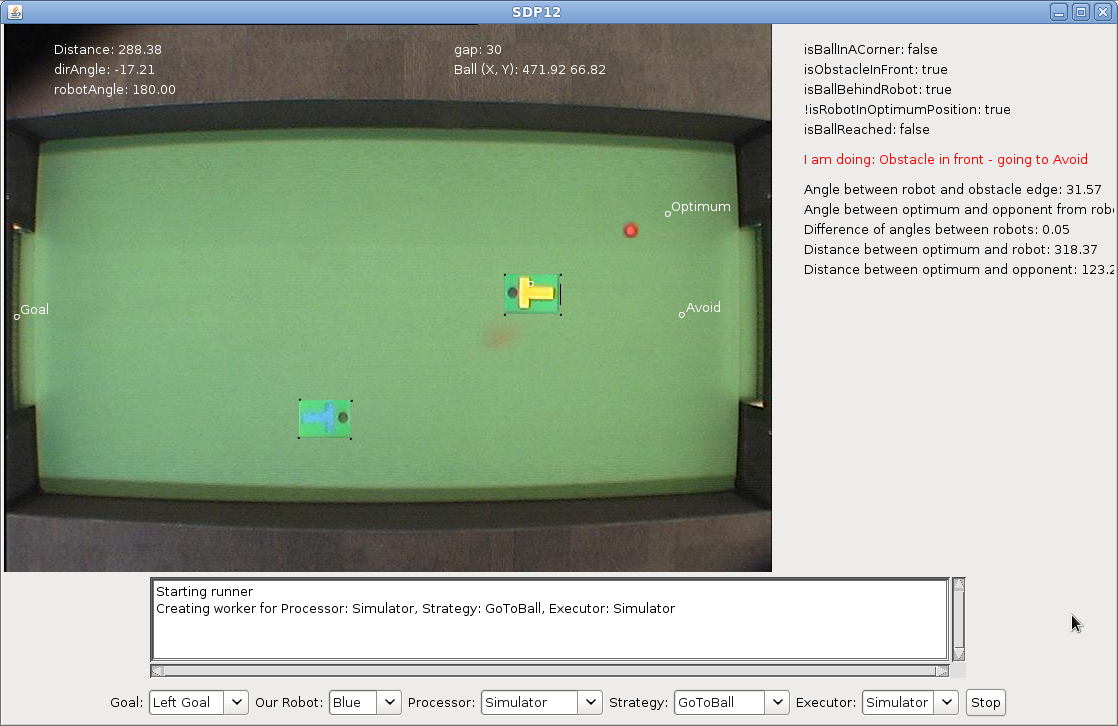
\includegraphics[width=0.8\textwidth] {GUI.png}
\end{center}
\label{fig:GUI}
\caption{Screenshot of GUI running the simulator}
\end{figure}
\begin{itemize}
 \item \textit{Goal}: Choose the goal that we are aiming at.
 \item \textit{Our Robot}: Determines if our robot is mounted with the blue or yellow plate.
 \item \textit{Processor}: Get the location information from either a file, a process (i.e. our vision system) or a simulator.
 \item \textit{Strategy}: A list of strategies including goToBall and takePenalty.
 \item \textit{Executor}: Execute the commands on the simulator or through Bluetooth.
\end{itemize}

\begin{figure}[htp]
\begin{center}
\leavevmode
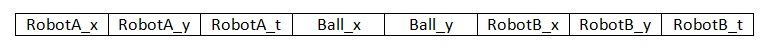
\includegraphics[width=0.8\textwidth] {vision.jpeg}
\end{center}
\caption{Data received from Vision}
\label{fig:visiondata}
\end{figure}

\cleardoublepage

\begin{algorithm}
\label{app:code}
\caption{GoToBall Strategy}
\begin{algorithmic}[1]
\WHILE {UpdateVision()}
	\STATE $left\gets 1$
	\STATE $right\gets 1$
	\STATE $threshold\gets 30$
	\STATE $requiredAngle\gets getAngleBetweenBallAndRobot()$
	\STATE $diffAngle\gets AngleOfRobot() - requiredAngle$
	\IF{diffAngle $<$ 0 AND abs(diffAngle) $<$ 180 OR 
		diffAngle $>$ 180 AND abs(diffAngle) $>$ 180}
		\STATE $right \gets -1$
		\STATE $left \gets 1$
	\ELSE
		\STATE $right \gets 1$
		\STATE $left \gets -1$
	\ENDIF
	\IF{abs(diffAngle) $<$ threshold}
		\STATE $right \gets distance$
		\STATE $left \gets distance$
	\ENDIF
	\STATE rotateWheels(right, left)
\ENDWHILE
\end{algorithmic}
\end{algorithm}


\end{document}
